\documentclass[10pt]{beamer}
\usepackage{graphicx}
\usepackage{amsmath}
\usepackage{bibentry}
\usepackage{biblatex}
\setbeamertemplate{caption}[numbered]
\bibliography{Bibliography}





\graphicspath{{images/}}
\setbeamertemplate{footline}[frame number]
\setbeamertemplate{page number in head/foot}[appendixframenumber]
\usetheme{Darmstadt}

\title[short]{INTELLIGENT SYSTEMS}
\author[Flavio Forenza]{Flavio Forenza \\ \tiny flavio.forenza@studenti.unimi.it\\[5mm] 
\includegraphics[scale = 0.06]{logoUnimi2.png}}
\institute{Department of Computer Science,\\ University of Milan, Italy}
\date{\tiny \today}

\begin{document}

\begin{frame}
    \maketitle
\end{frame}


\logo{
\includegraphics[width=0.1\linewidth]{logoUnimi2.png}}
\section{Paper 1}
\subsection{\emph{"A Unified Framework for Salient StructureDetection by Contour-Guided Visual Search"}}
\begin{frame}{INTRODUCTION}
    The purpose of the paper is to introduce a new method, called CGVS in the 
    state of the art, which is able to identify regions and salient objects 
    within a scene simultaneously. The proposed system attempts to 
    bridge the gap between the two highly related tasks of \emph{"human 
    fixation"} prediction and \emph{"salient object detection"}, with a general 
    framework.
\end{frame}

\begin{frame}{RELATED WORK}
    To obtain the final result, two pathways are crossed (Fig.\ref{fid: flowchart}):
    \begin{enumerate}
        \item Selective
        \item Non-Selective
    \end{enumerate}
    \begin{figure}[htbp]
        \centering
        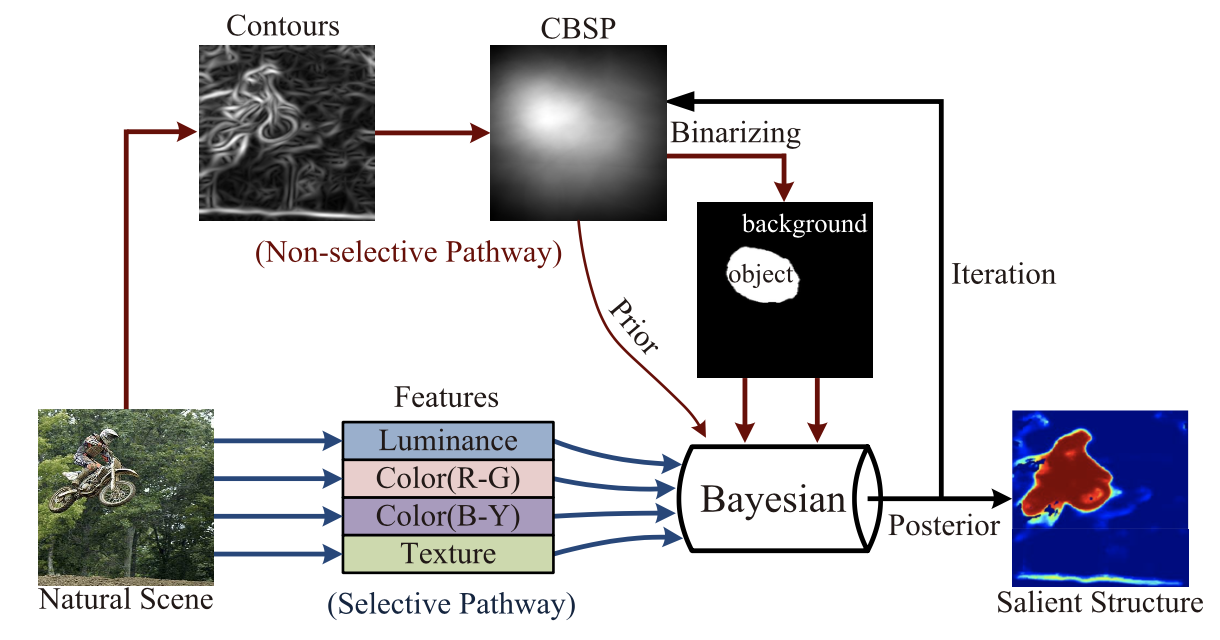
\includegraphics[width = 0.8\linewidth]{images/paper1/selective and non-selective pathways.png}
        \centering
        \caption{The flowchart of the porposed system.}
        \label{fid: flowchart}
    \end{figure}
\end{frame}

\begin{frame}[t]{CONTOUR-GUIDED VISUAL SEARCH MODEL pt1}
    In \emph{Non-Selective} pathway are computed:
    \begin{enumerate}
        \item \emph{Boundary} \footfullcite{0747815570}
        \item \emph{Contour-Based Spatial Prior (CBSP)} $ \rightarrow S_w = S_e + S_c $
    \end{enumerate}
    \begin{figure}[htbp]
        \centering
        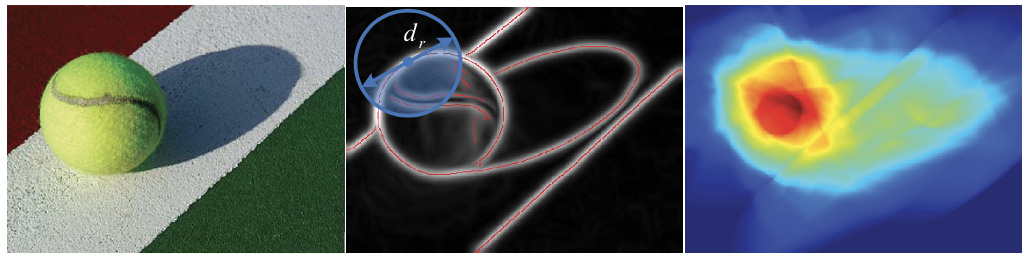
\includegraphics[width = 0.5\linewidth]{images/paper1/CBSP.png}
        \centering
        \caption{CBSP reconstruction.}\vspace{0mm}
        \label{fid: CBSP}
    \end{figure}
    In \emph{Selective} pathway are computed the basic low-level features:
    \begin{enumerate}
        \item \emph{Luminance} $ \rightarrow f_{lum} = (r+g+b)/3 $
        \item \emph{Color-Opponent} $ \rightarrow f_{rg} = r-g , f_{by} = b-(r+g)/2 $
        \item \emph{Texture Channel} ($ f_{ed} $)
    \end{enumerate}
\end{frame}

\begin{frame}[t]{CONTOUR-GUIDED VISUAL SEARCH MODEL pt2}
    \begin{block}{Bayesian inference}
        All the previous informations are used to compute the Bayesian inference:
        $$ p(s|x) = \frac{p(s)p(x|s)}{p(s)p(x|s)+p(b)p(x|b) } $$
    \end{block}
    Where:
    \begin{enumerate}
        \item $ p(x|s) \rightarrow $ likelihood of a pixel at \emph{x} belonging to a salient structure \emph{s}
        \item $ p(x|b) \rightarrow $ likelihood of a pixel at \emph{x} belonging to the background \emph{b}
        \item $ p(s) \mbox{ and } p(b)=1-p(s) \rightarrow $ prior probabilities of a pixel at x belonging to a salient structure and the background, respectively.
    \end{enumerate}
\end{frame}

\begin{frame}{CONTOUR-GUIDED VISUAL SEARCH MODEL pt3}
    To compute the prior probabilities, we need:
    \begin{enumerate}
        \item \emph{Predict the Size of Potential Structure}: using a optimal threshold ($ T_{opt} $) 
        useful for separating the background from the foreground (salient structures).
        \item \emph{Evaluate the Importance of Each Feature}: weighing every salient structure.
        \item \emph{Calculate the Observation Likelihood:} both $ p(x|s) \mbox{ and } p(x|b) $
        \item \emph{Enhance the Salient Structure by Iterating}: we re-initialize the prior 
        function with the smoothed version of $ p(s|x) $ (by median filtering 
        with a size of 21 × 21 pixels)
    \end{enumerate}
\end{frame}

\begin{frame}[t]{EXPERIMENTS}
    The results obtained on different datasets \footfullcite{PASCAL-S, ECSSD, ASD}, were compared with those 
    btained by the systems already existing at the state of the art.
    \begin{figure}[htbp]
        \centering
        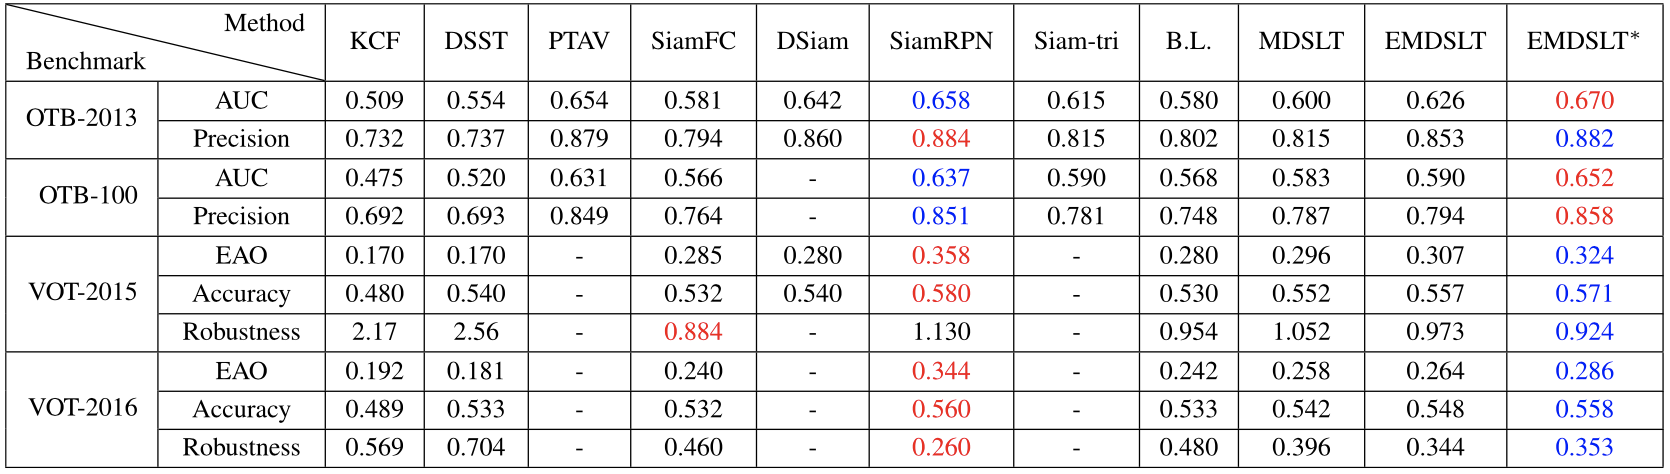
\includegraphics[width = 0.8 \linewidth]{/paper1/metrics.png}
        \centering
        \caption{Metrics comparison.}
        \label{fig: metrics}
    \end{figure}
\end{frame}

\begin{frame}{DISCUSSION}
    It is necessary to say that the results obtained by the proposed method 
    are obtained using the center bias, which if removed places the system 
    performance under those of systems such as \emph{RF} \footfullcite{0747815518} and \emph{HS}\footfullcite{0747815508} (which do not 
    use the central bias). This method offers a dual use. In 
    a cluttered scene with no dominant objects, the system will function as a 
    fixation prediction model. Finally, on the other hand, with simple scenes, 
    the system detects existing relevant objects.
    \begin{figure}[htbp]
        \centering
        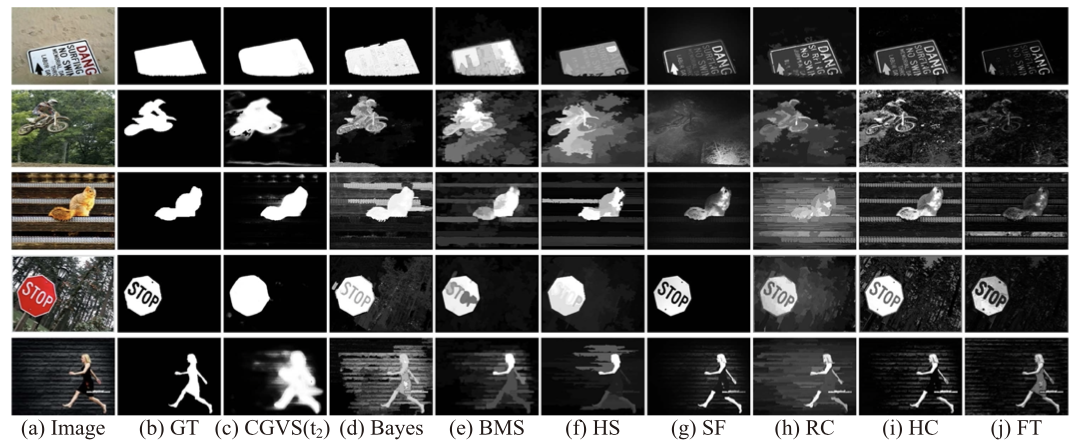
\includegraphics[width = 0.7 \linewidth]{paper1/SystemsComp.png}
        \centering
        \label{fig: metrics}
    \end{figure}
\end{frame}

\section{Paper 2}
\begin{frame}
    
\end{frame}




    
\end{document}
